\section{Experimental procedure}
\subsection{Adjusting the gain of the Amplifier}
First, we adjusted the gain of both amplifiers  ($A_{1}$ and  $A_{2}$) during the set up of the experiment.We visualized the signal with the help of Oscilloscope. Following figure shows the amplified signal from the Amplifier1.
\begin{figure}[ht]
	\centering
	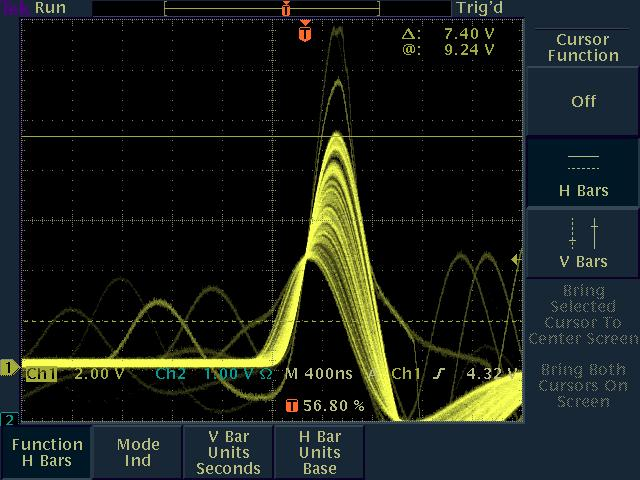
\includegraphics[width=0.8\linewidth]{./figs/amplified.jpg}
	\caption{Amplified Signal Output from the Detector.}%
	\label{fig:angAsymm}
\end{figure}

\subsection{Adjusting of the CFD}
CFD has a threshold-discriminator which help to filter out zero crossing that belongs to electronic noise and not to a true scintillation signal. So, we have adjusted this threshold of CFD to detect only true signals not the background noise signals. In that step, We connected the negative outputs of the both CFDs to the counters and measured the count rates with and without source installed.

\subsection{Setting up the Fast Coincidence}
In this step, we visualized the coincidence of incoming signals from two CFDs with th help of oscilloscope and then determined the proper delay.For that, we connected the negative outputs of both CFDs to the oscilloscope and triggered on the first channel signals.Then, on the second channel, true coincidence appeared. Then, we inserted the fixed delay in between CFD1 and FC and a variable delay in between CFD2 and FC. After that, we picked the resolving time for FC as 25 ns.

\subsection{Setting up the Slow Coincidence}
Here, we connected the output from the fast coincidence unit to a gate and delay ($ D^{2}-G^{2} $) generator module. Also, the delay of both SCAs can be adjusted. Then, the output from ($ D^{2}-G^{2} $) inserted to the first channel and positive output from SCA1 and SCA2 on after another to th second channel of the oscilloscope. Afterward, we adjusted the delays in both SCAs and ($ D^{2}-G^{2} $). 

\subsection{Calibrating th Signal Channel Analyzer}
In this step, we performed the energy calibration and recorded the energy spectrum by using SCAs. For that, we set the SCA to the window mode. Later  we keep thee constant obtained window width for our measurement. Figure 7 and figure 8 shows the energy spectrum of $ ^{60}Co$-decay obtained by SCA1 and SCA2 respectively.
\begin{figure}[ht]
	\centering
	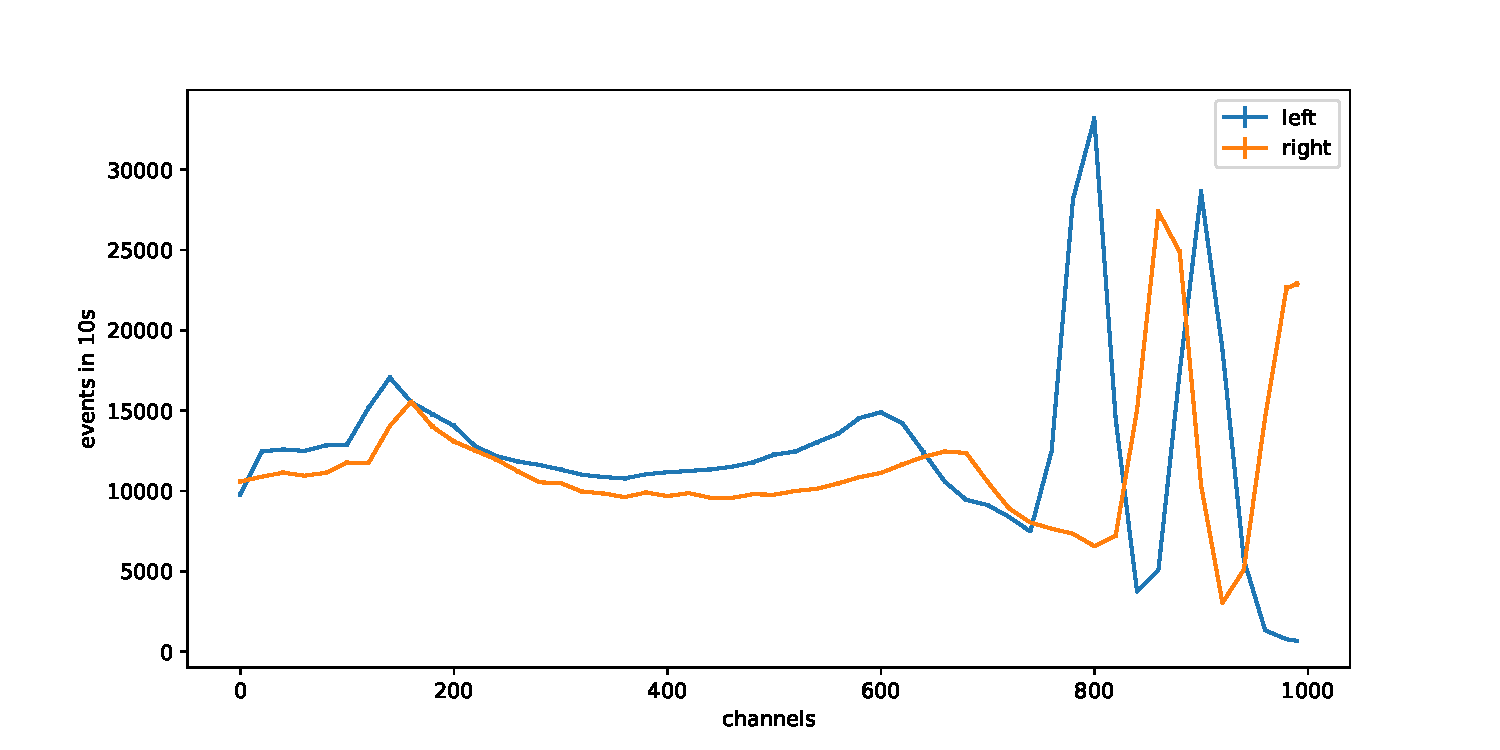
\includegraphics[width=0.8\linewidth]{./figs/sca.pdf}
	\caption{The energy spectra of SCA1. Here two peaks are in the range of [750-1000].}%
	\label{fig:angAsymm}
\end{figure}

\begin{figure}[ht]
	\centering
	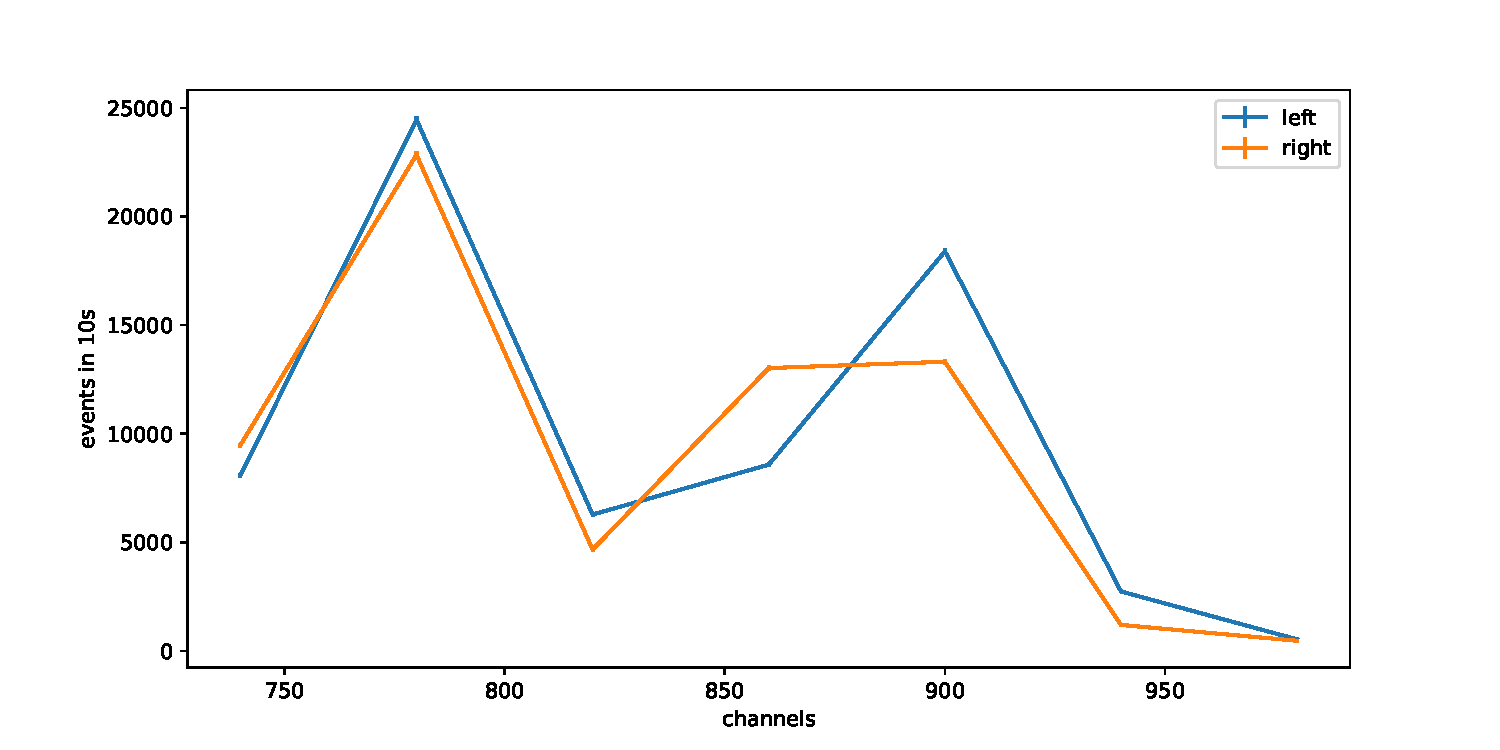
\includegraphics[width=0.8\linewidth]{./figs/sca2.pdf}
	\caption{The energy spectra of SCA2. Here two peaks are in the range of [750-950].}%
	\label{fig:angAsymm}
\end{figure}


\subsection{Main Measurement}
After adjusting all the involving apparatus in the experiment, we stated to perform th main measurement of the experiment. we used two detectors: on of them is fixed and another is movable. We inserted both detectors 5cm apart from the source. Then we measured the count rates for different angles between these two detectors.



